\section{Introduction}
\frame{
  \frametitle{Stub}
}
\frame{
  \frametitle{Publications}
  \cite{NRSFMpaper}

}
\section{Structured Light}
\frame{
  \frametitle{Stub}
}
\section{Non-Rigid Structure from Motion}
\frame{
  \frametitle{Concept}
  Take a series of $P$ 2D observations over $F$ frames...
  \begin{center}
    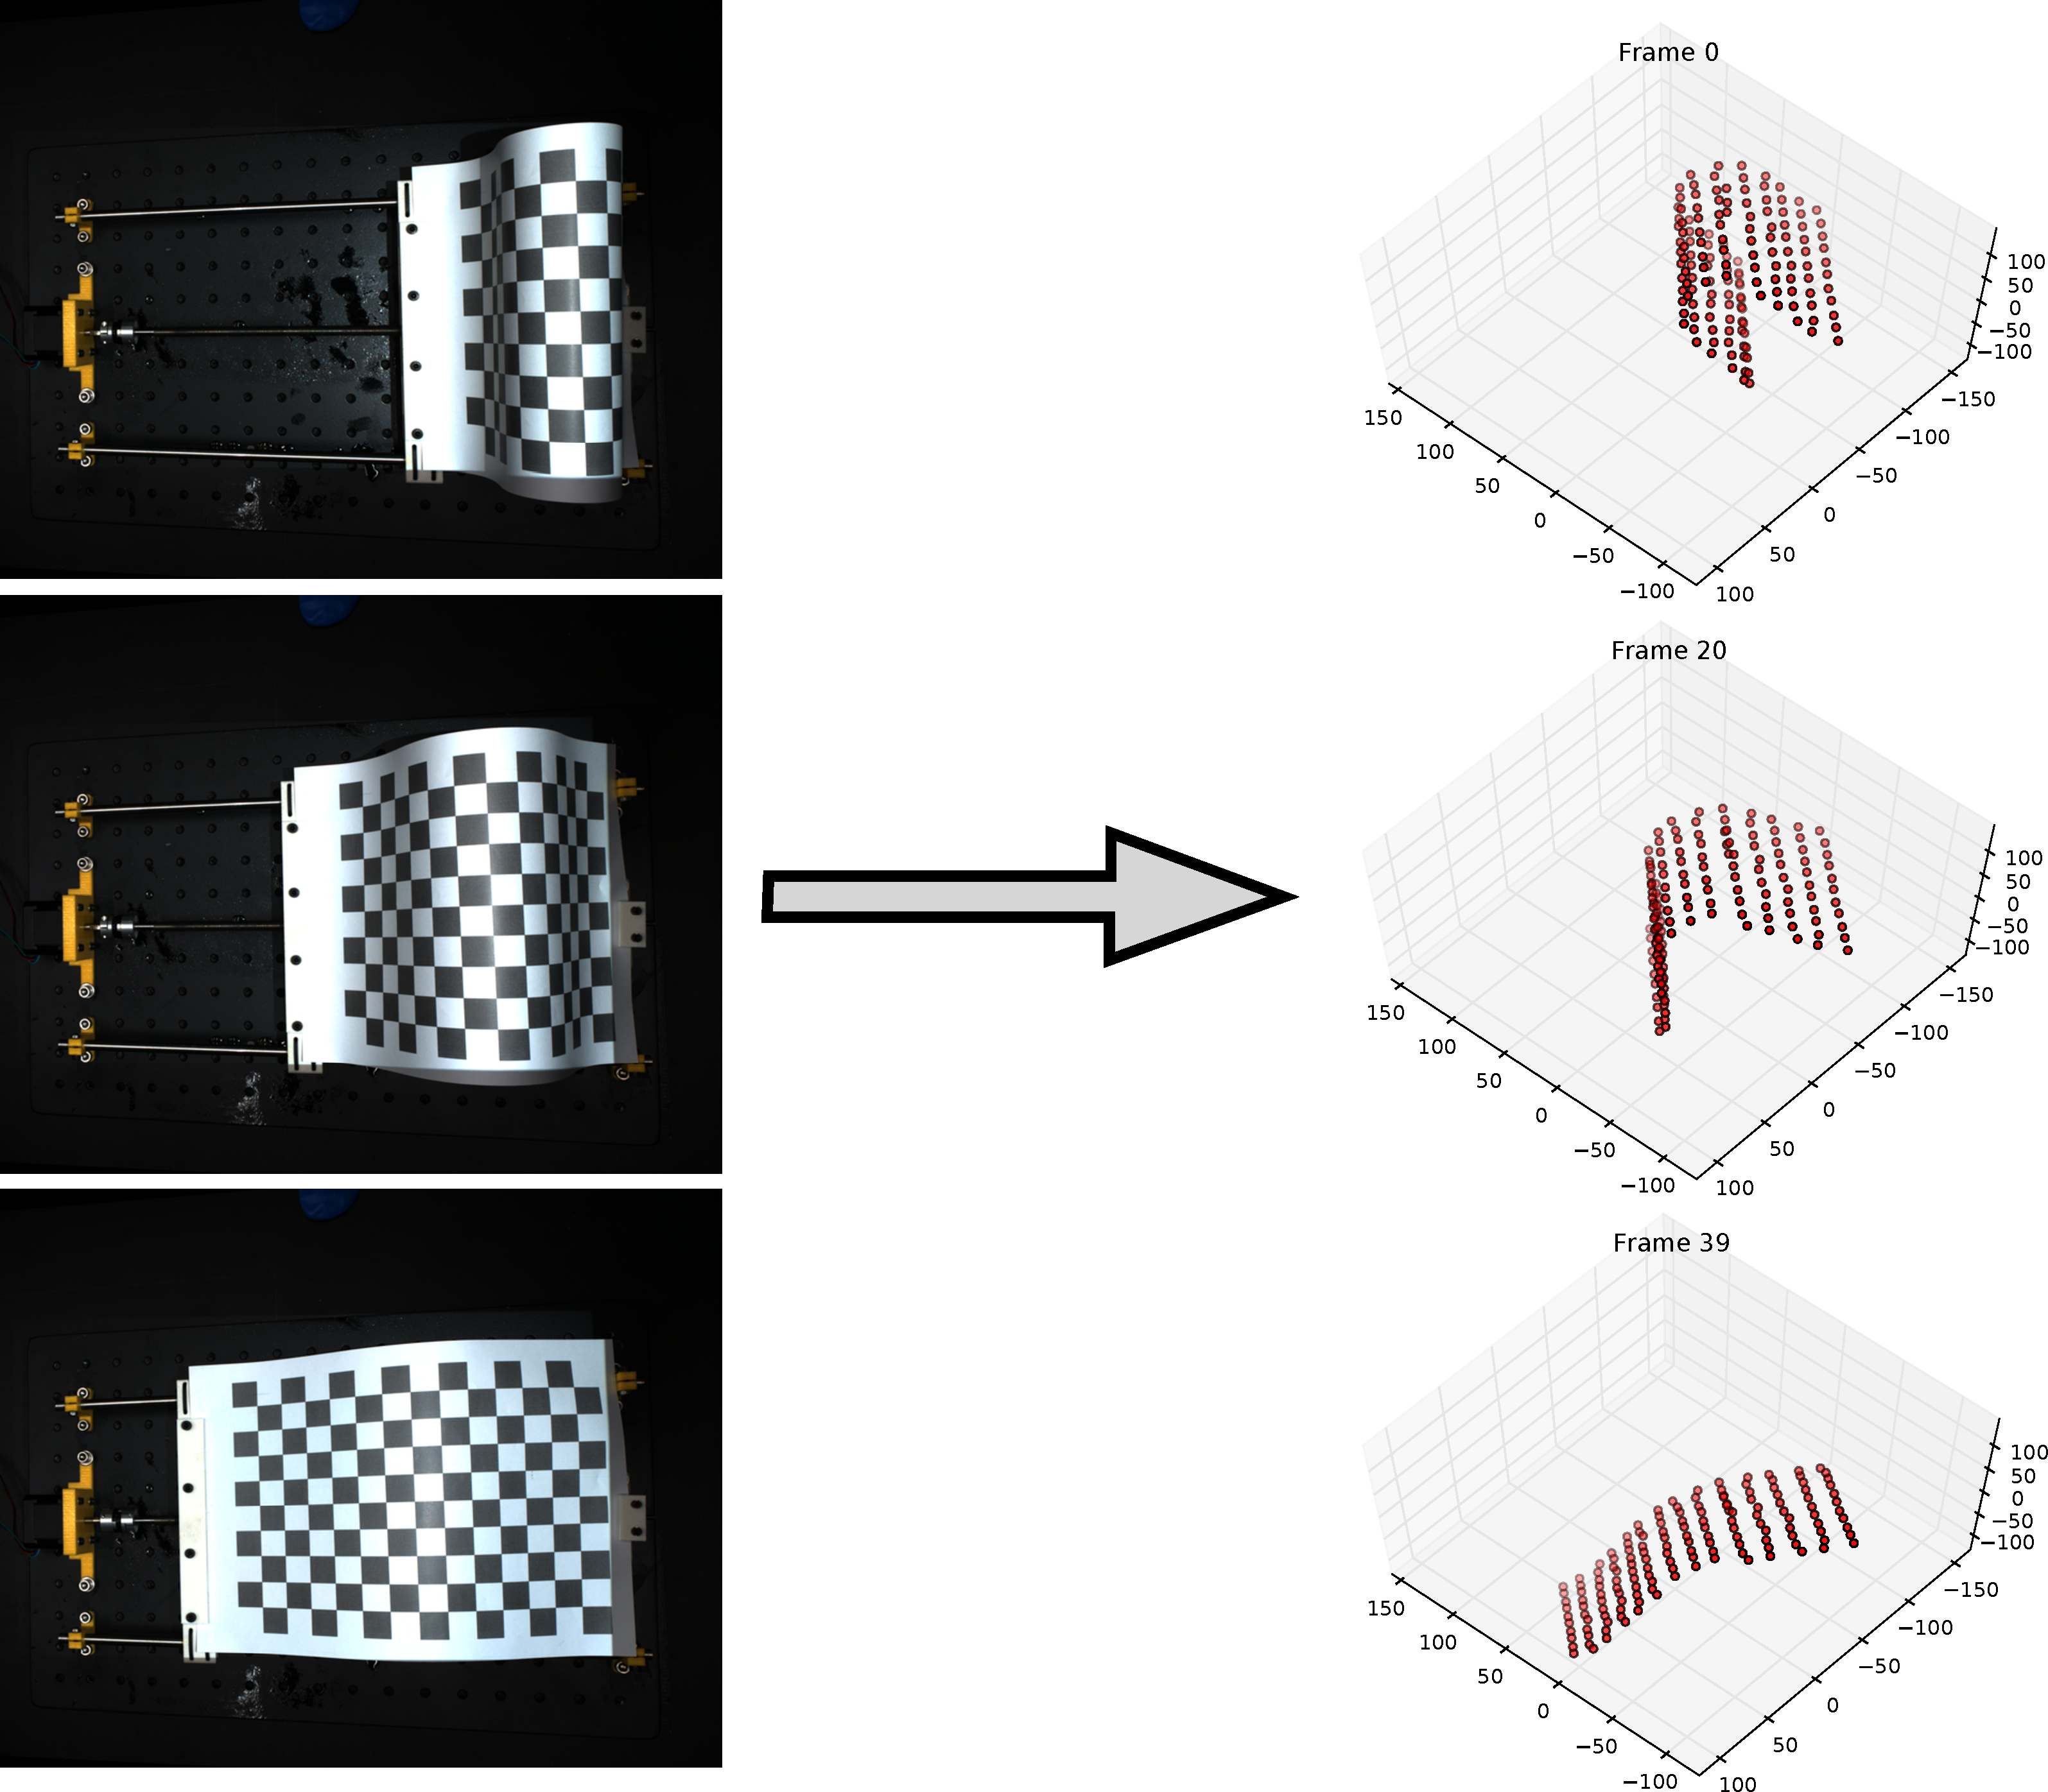
\includegraphics[width=0.4\textwidth]{figures/nrsfm_paper_idea}
  \end{center}
  ...and estimate 3D geometry.
}

\frame{
  \frametitle{Factorization}
  Factorize observations $\mathbf{W}$ into camera $\mathbf{M}$ and geometry components $\mathbf{S}$,
  \begin{align}
    \mathbf{W} = \mathbf{M}\mathbf{S}    \label{eq:nrsfm_fac}
  \end{align}
  \begin{align*}
    \mathbf{W} = \begin{bmatrix}
      \mathbf{w}_{11} & \mathbf{w}_{12} & \cdots & \mathbf{w}_{1P}\\
      \mathbf{w}_{21} & \mathbf{w}_{22} & \cdots & \mathbf{w}_{2P}\\
      \vdots   & \vdots   & \ddots & \vdots\\
      \mathbf{w}_{F1} & \mathbf{w}_{F2} & \cdots & \mathbf{w}_{FP}
    \end{bmatrix},
    \mathbf{M} = \begin{bmatrix}
      \mathbf{M}_1 & \mathbf{0}   & \cdots & \mathbf{0}\\
      \mathbf{0}   & \mathbf{M}_2 & \cdots & \mathbf{0}\\
      \vdots       & \vdots       & \ddots & \vdots    \\
      \mathbf{0}   & \mathbf{0}   & \cdots & \mathbf{M}_F
    \end{bmatrix},
    \mathbf{S} = \begin{bmatrix}
      \mathbf{s}_{11} & \mathbf{s}_{12} & \cdots & \mathbf{s}_{1P}\\
      \mathbf{s}_{21} & \mathbf{s}_{22} & \cdots & \mathbf{s}_{2P}\\
      \vdots       & \vdots       & \ddots & \vdots    \\
      \mathbf{s}_{F1} & \mathbf{s}_{F2} & \cdots & \mathbf{s}_{FP}
    \end{bmatrix}
  \end{align*}
  Here we assume that $\mathbf{M}_f$ is an orthographic projection matrix.
}

\frame{
  \frametitle{Low-Rank Basis}
  An often assumed prior is that deformation can be expressed as a linear combination of a set of $K$ basis vectors,
  \begin{align}
    \mathbf{s}_f = c_{f, 1}\mathbf{b}_1 + c_{f, 2}\mathbf{b}_2 + \cdots +
                    + c_{f, K}\mathbf{b}_K.
  \end{align}
  Expressed in terms of the factorization problem from \eqref{eq:nrsfm_fac}.
  \begin{align}
    \mathbf{W} = \mathbf{M}\underbrace{(\mathbf{C} \otimes \mathbf{I}_3)
      \begin{bmatrix}
        \mathbf{b}_1 & \mathbf{b}_2 & \cdots & \mathbf{b}_K
      \end{bmatrix}^\text{T}
    }_\mathbf{S}\label{eq:nrsfm_lowrank},
        \mathbf{C} = \begin{bmatrix}
      c_{1, 1} & c_{1, 2} & \cdots & c_{1, K}\\
      c_{2, 1} & c_{2, 2} & \cdots & c_{2, K}\\
      \vdots & \vdots & \ddots & \vdots\\
      c_{F, 1} & c_{F, 2} & \cdots & c_{F, K}\\
    \end{bmatrix}
  \end{align}
}
